\documentclass[border=6pt]{standalone}
\usepackage{pgfplots}
\pgfplotsset{compat=1.18}
\begin{document}
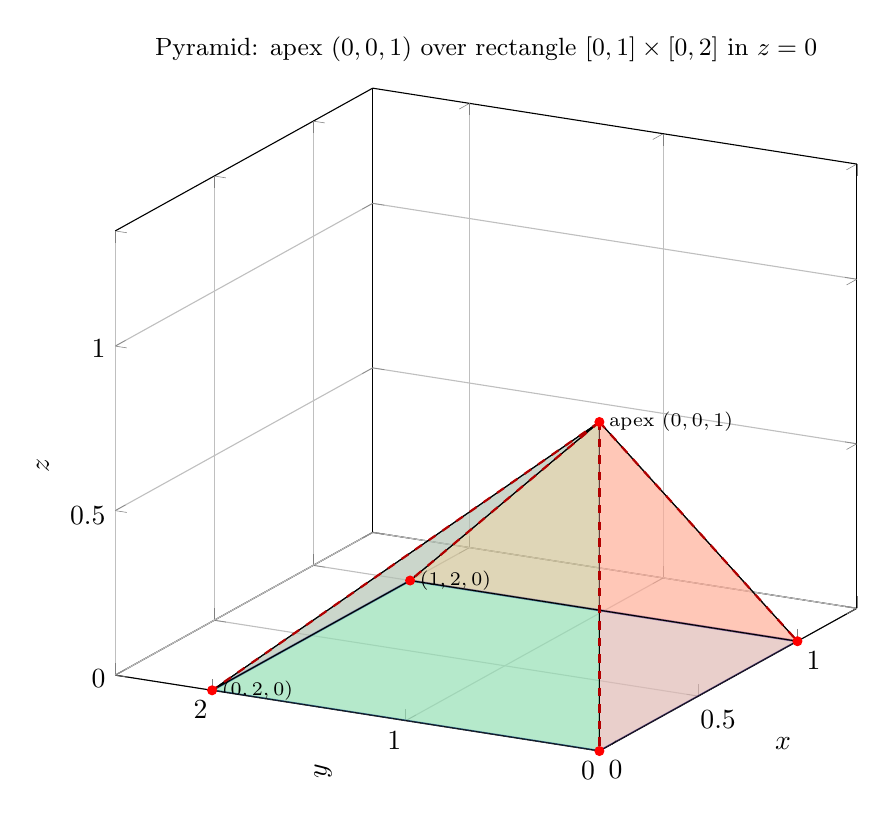
\begin{tikzpicture}
\begin{axis}[
    view={-62}{20},
    width=11cm, height=10cm,
    xlabel=$x$, ylabel=$y$, zlabel=$z$,
    xmin=0, xmax=1.3,
    ymin=0, ymax=2.5,
    zmin=0, zmax=1.35,
    xtick={0,0.5,1}, ytick={0,1,2}, ztick={0,0.5,1},
    axis lines=box,
    grid=major,
    title={\small Pyramid: apex $(0,0,1)$ over rectangle $[0,1]\times[0,2]$ in $z=0$},
]
% base rectangle z=0
\addplot3[fill=blue!35, fill opacity=0.45, draw=blue!60!black, thick]
  coordinates {(0,0,0) (1,0,0) (1,2,0) (0,2,0)} -- cycle;
% face y=0
\addplot3[fill=orange!45, fill opacity=0.45, draw=black]
  coordinates {(0,0,0) (1,0,0) (0,0,1)} -- cycle;
% face x=0
\addplot3[fill=green!45, fill opacity=0.45, draw=black]
  coordinates {(0,0,0) (0,2,0) (0,0,1)} -- cycle;
% face x+z=1
\addplot3[fill=red!40, fill opacity=0.40, draw=black]
  coordinates {(1,0,0) (0,0,1) (1,2,0)} -- cycle;
% face y+2z=2
\addplot3[fill=violet!40, fill opacity=0.40, draw=black]
  coordinates {(1,2,0) (0,2,0) (0,0,1)} -- cycle;
% edges from apex
\addplot3[draw=red!70!black, thick, dashed, mark=none]
  coordinates {(0,0,1) (0,0,0)};
\addplot3[draw=red!70!black, thick, dashed, mark=none]
  coordinates {(0,0,1) (1,0,0)};
\addplot3[draw=red!70!black, thick, dashed, mark=none]
  coordinates {(0,0,1) (1,2,0)};
\addplot3[draw=red!70!black, thick, dashed, mark=none]
  coordinates {(0,0,1) (0,2,0)};
% vertices
\addplot3[only marks, mark=*, mark size=1.6pt, color=red] coordinates {
 (0,0,0) (1,0,0) (1,2,0) (0,2,0) (0,0,1)};
\node[anchor=west] at (axis cs:0,0,0) {\scriptsize $(0,0,0)$};
\node[anchor=west] at (axis cs:1,-0.15,0) {\scriptsize $(1,0,0)$};
\node[anchor=west] at (axis cs:1,2,0) {\scriptsize $(1,2,0)$};
\node[anchor=west] at (axis cs:0,2,0) {\scriptsize $(0,2,0)$};
\node[anchor=west] at (axis cs:0,0,1) {\scriptsize apex $(0,0,1)$};
\end{axis}
\end{tikzpicture}
\end{document}
